\section{Feeding Strategies}\label{sec:prediction-strategies}
To solve the problem of visual odometry, we tried different approaches to feed the sequence of image into the model, and to construct the model itself.
We tried following approaches to feed the data:
\begin{enumerate}
    \item Feeding the sequence into the model directly and presenting the pose as \emph{euler angles}.
    \item Feeding the sequence into the model directly and presenting the pose as \emph{rotation matrix} so with twelve numbers and \emph{translation vector}.
    \item Feeding the sequence into the model where the first frame is the origin of the reference frame and presenting the pose as \emph{euler angles}.
    \item Feeding the sequence into the model where the first frame is the origin of the reference frame and presenting the pose as \emph{rotation matrix} and \emph{translation vector}.
    \item Feeding the sequence into the model where the first frame is the origin of the reference frame, and using the auto-regressive model to predict the pose.
\end{enumerate}
We can divide these strategies into two groups: the first group is composed by strategy 1 and 2, and the second group is composed by strategy 3, 4 and 5.
This division is because the first group uses the ground-truth without any preprocessing, meanwhile the second group uses the ground-truth translated with respect to the first pose of the sequence.

\subsection{Directly feeding the sequence}\label{subsec:directly-feeding-the-sequence}
With this strategy, we create each sequence by taking the images from the dataset and the pose as ground-truth without any processing.
For the sake of simplicity, to explain the different strategy, we will use an example of trajectory which is as represented in the Figure 4.6:
\begin{figure}[H]
    \centering
    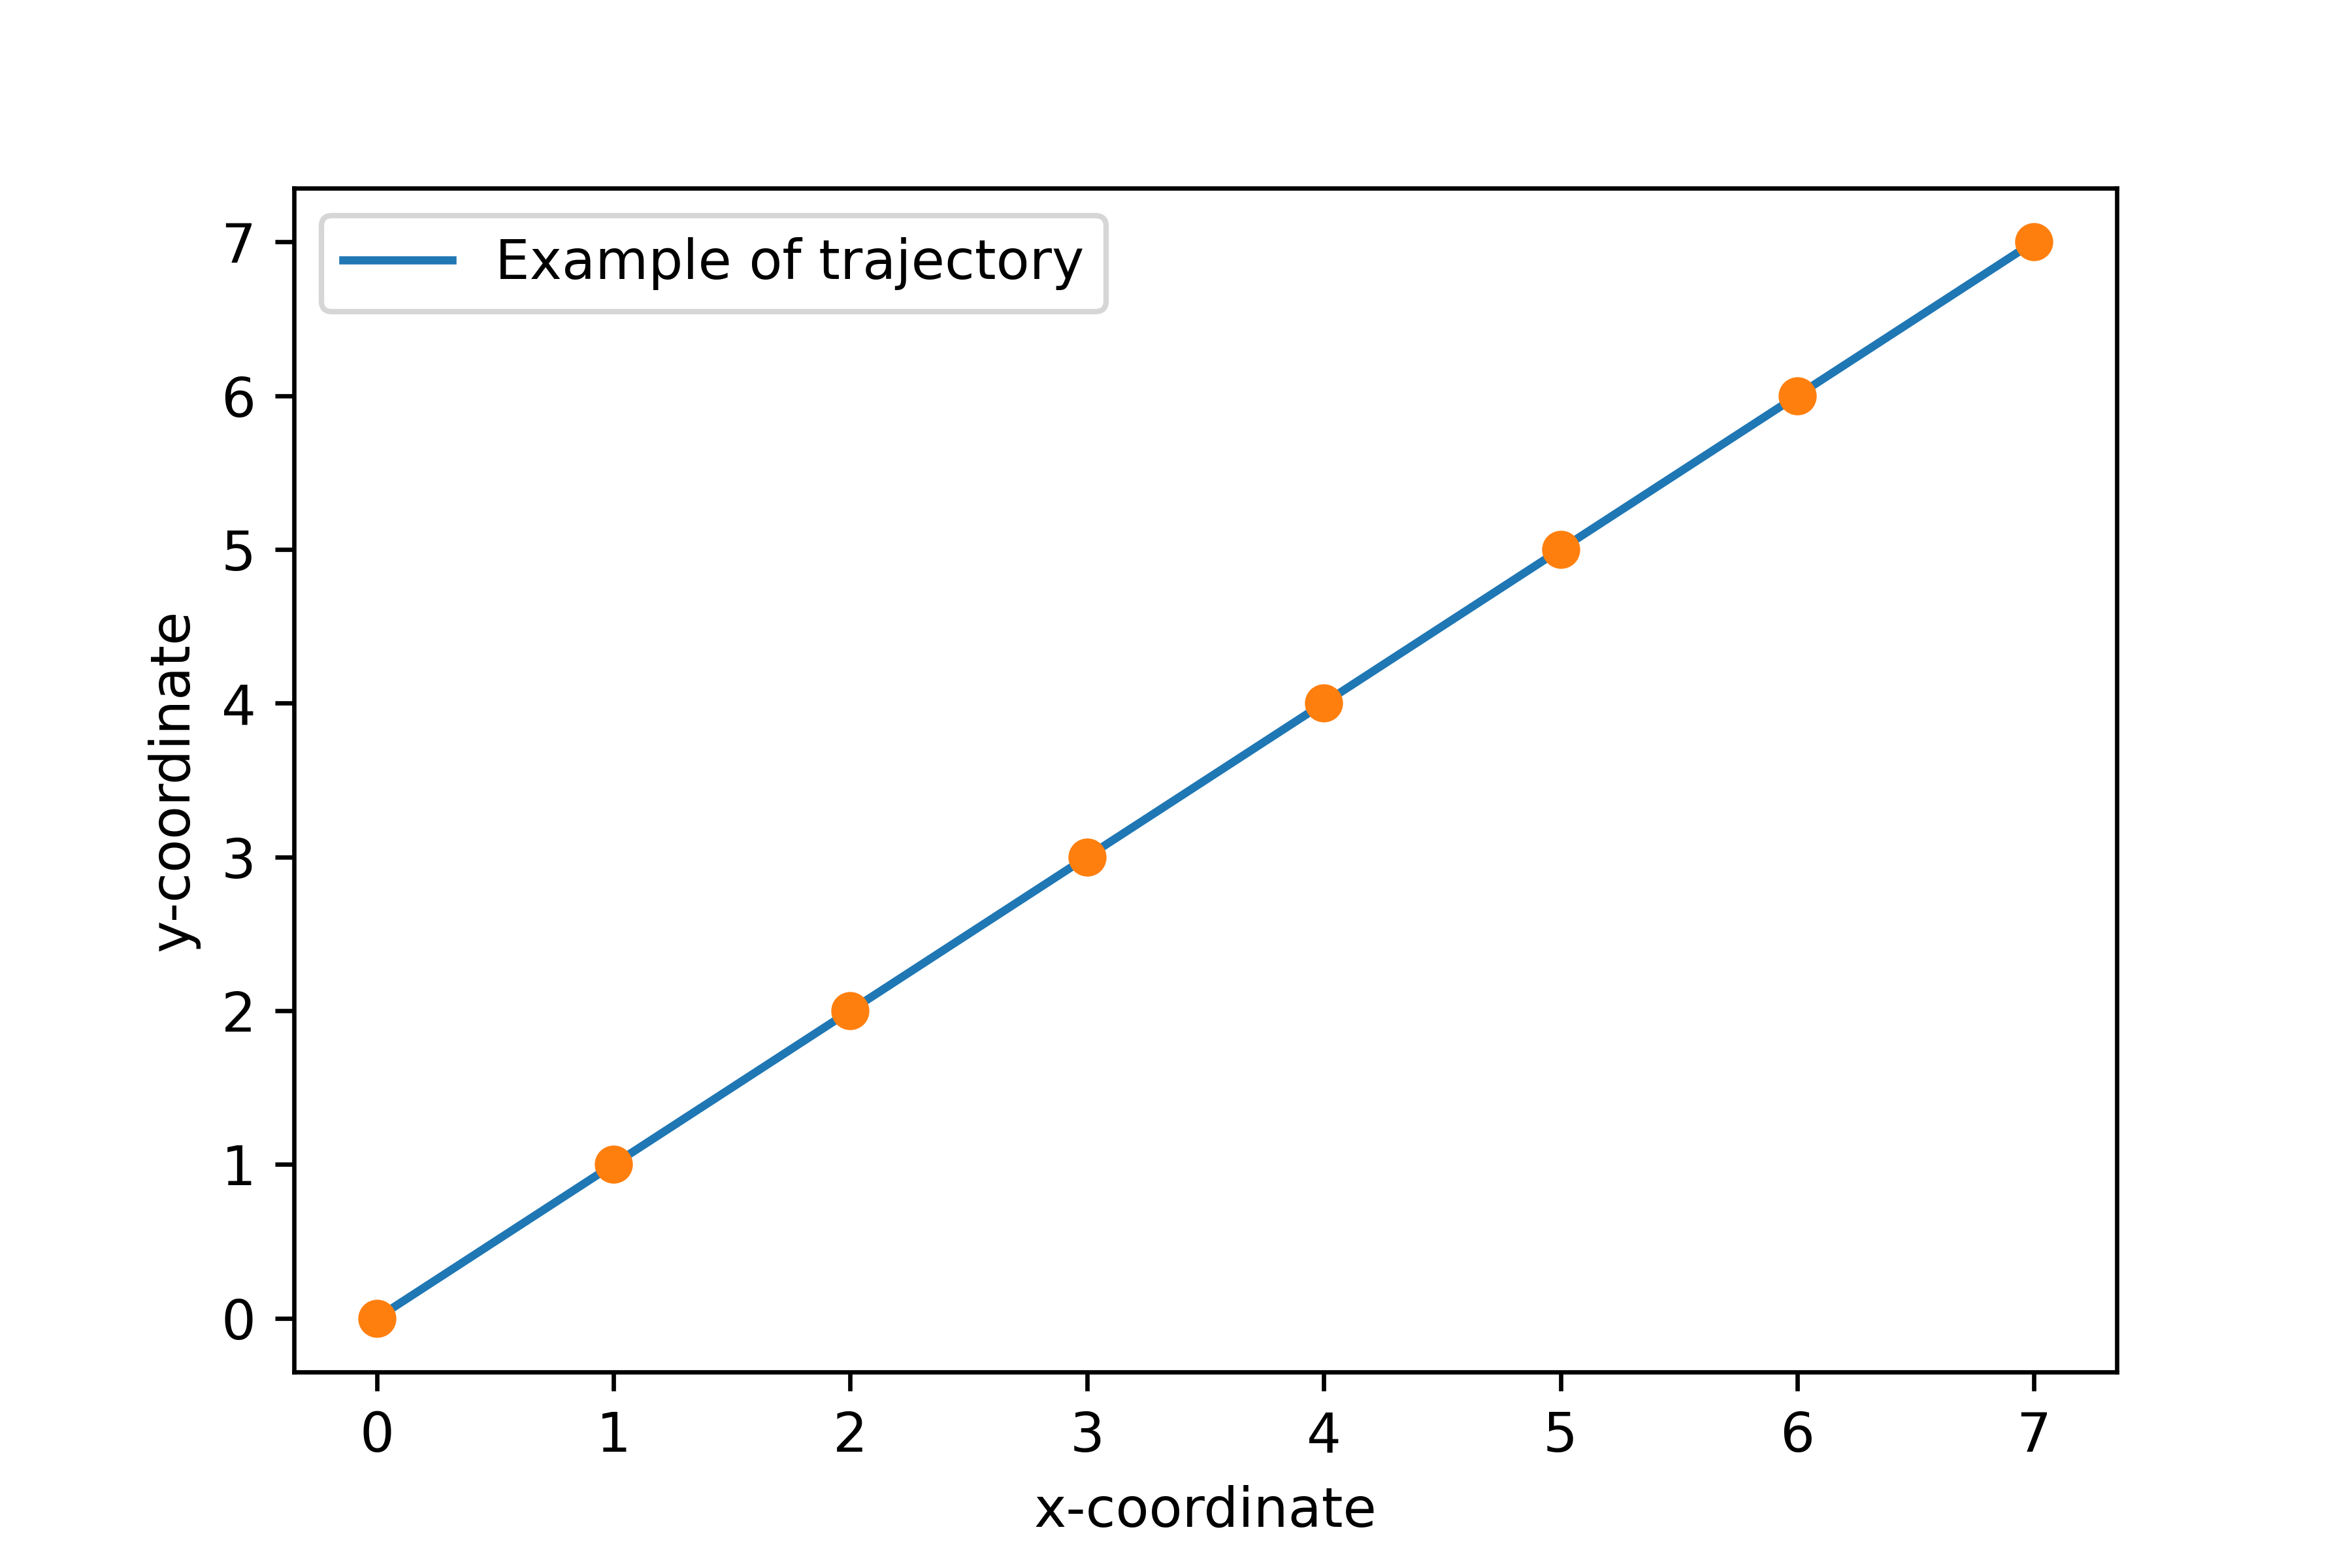
\includegraphics[width=\textwidth]{images/4_2_example_of_trajectory}
    \caption{Example of the trajectory.}
    \label{fig:example-of-trajectory}
\end{figure}
Of course, in the example the trajectory looks easy to predict because the distance between every pair of pose is the same, and trajectory direction is not changing.
Meanwhile, in the KITTI dataset, the trajectories are more complex, and the distance between the poses is not constant, and the direction of the trajectory is changing.
We can see the trajectory where each dot represents an image-pose pair.
From this trajectory, we can represent the dataset and  the creation of the sequences as follows:
\begin{figure}[H]
    \centering
    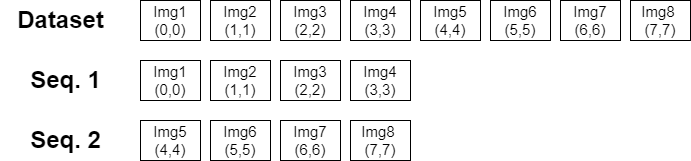
\includegraphics[width=\textwidth]{images/4_2_directly_feeding}
    \caption{Example of the dataset.}
    \label{fig:example-of-dataset}
\end{figure}
This way of feeding the data is the simplest one, but it has some drawbacks.
The first one is that when we split the training dataset into different sequences, for each sequence, the coordinates do not start from the origin (i.e., (0,0)) but for example for the second sequence, it starts from (4,4).
This is problematic for the model because it has to learn this kind of translation, and it is not a trivial task.
The second drawback is that the model has to predict a very large interval of numbers in this case, the range goes from 0 to 7, but in real case, like in the KITTI dataset, the range goes from 0 to 1000.
The third drawback is that, with a dataset of $N$ images, we can have only $\frac{N}{seq\_len}$ sequences, where $seq\_len$ is the length of the sequence, this aggravates on the problem of small dataset available.


\subsection{Sequence with origin}\label{subsec:sequence-with-origin}
In this second strategy, we create each sequence by taking the images from the dataset, and the pose as ground-truth by performing a translation operation.
In this way, the sequences can be represented as follows:
\begin{figure}[H]
    \centering
    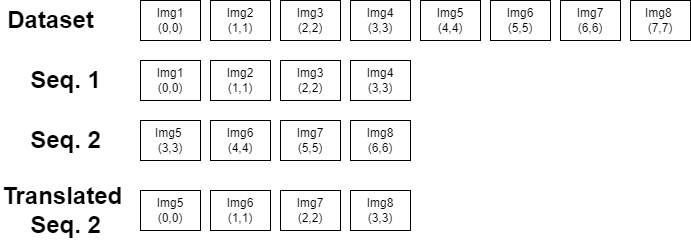
\includegraphics[width=\textwidth]{images/4_2_split_traj_1}
    \caption{Example of the dataset with origin.}
    \label{fig:example-of-dataset-with-origin}
\end{figure}
We can see that the sequences start from the origin, and the model has to learn only the relative pose to the first frame of the sequence, instead of the whole trajectory.
But this solution is not perfect, in the sense that, in this trajectory we have eight image-pose pair, and with $seq_len = 4$ we can generate only two sequences, and considering that the Kitti dataset has about 20.000 images, this is a big problem.

To solve the previous mentioned problem, we devised a slightly modified strategy, which essentially takes every image-pose pair and creates a sequence of length $seq\_len$, like represented in Figure 4.9:
\begin{figure}[H]
    \centering
    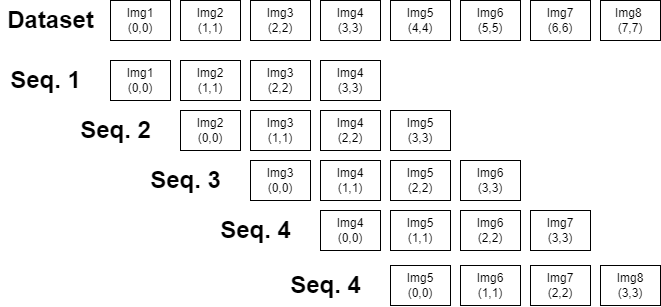
\includegraphics[width=\textwidth]{images/4_2_split_traj_2}
    \caption{Example of the dataset with origin.}
    \label{fig:example-of-dataset-with-origin-2}
\end{figure}
As represented in the previous figure, with a dataset of $N$ images, we can have $N - seq\_len +1 $ sequences, and this is a big improvement with respect to the previous strategy.
Also, in this way, we are doing a sort of data augmentation, because we're feeding the model with different sequences, and this is helpful for the model.

As comparison, with first strategy, using KITTI dataset, we can have only $\frac{N}{seq\_len}$ sequences, where $N = 20.000$ and $seq\_len = 4$, so we can have only $5000$ sequences, while with the latest strategy, we can have $N - seq\_len +1$ sequences, so we can have $19997$ sequences, which is an important improvement.
